\documentclass[a4paper ,12pt, onecolumn]{article}
\usepackage[utf8]{inputenc}
\usepackage[spanish]{babel}

\usepackage[hidelinks]{hyperref}
\usepackage{graphicx}
\graphicspath{ {./images/} }


\begin{document}

\title{Sistemas de posicionamiento de objetos mediante tecnología Bluetooth Low Energy
Beacon }
\author{Rubén Arce}
\date{\today}
\maketitle
\tableofcontents
\cleardoublepage
\section{Memoria descriptiva}
Antecedentes, objeto, normativa, reglamentación
Extensión máxima de 30 páginas + anexos 60
Defensa de 20 min  40
\section{Memoria justificativa}
\paragraph{hola}
asdfasd
\paragraph{}
a
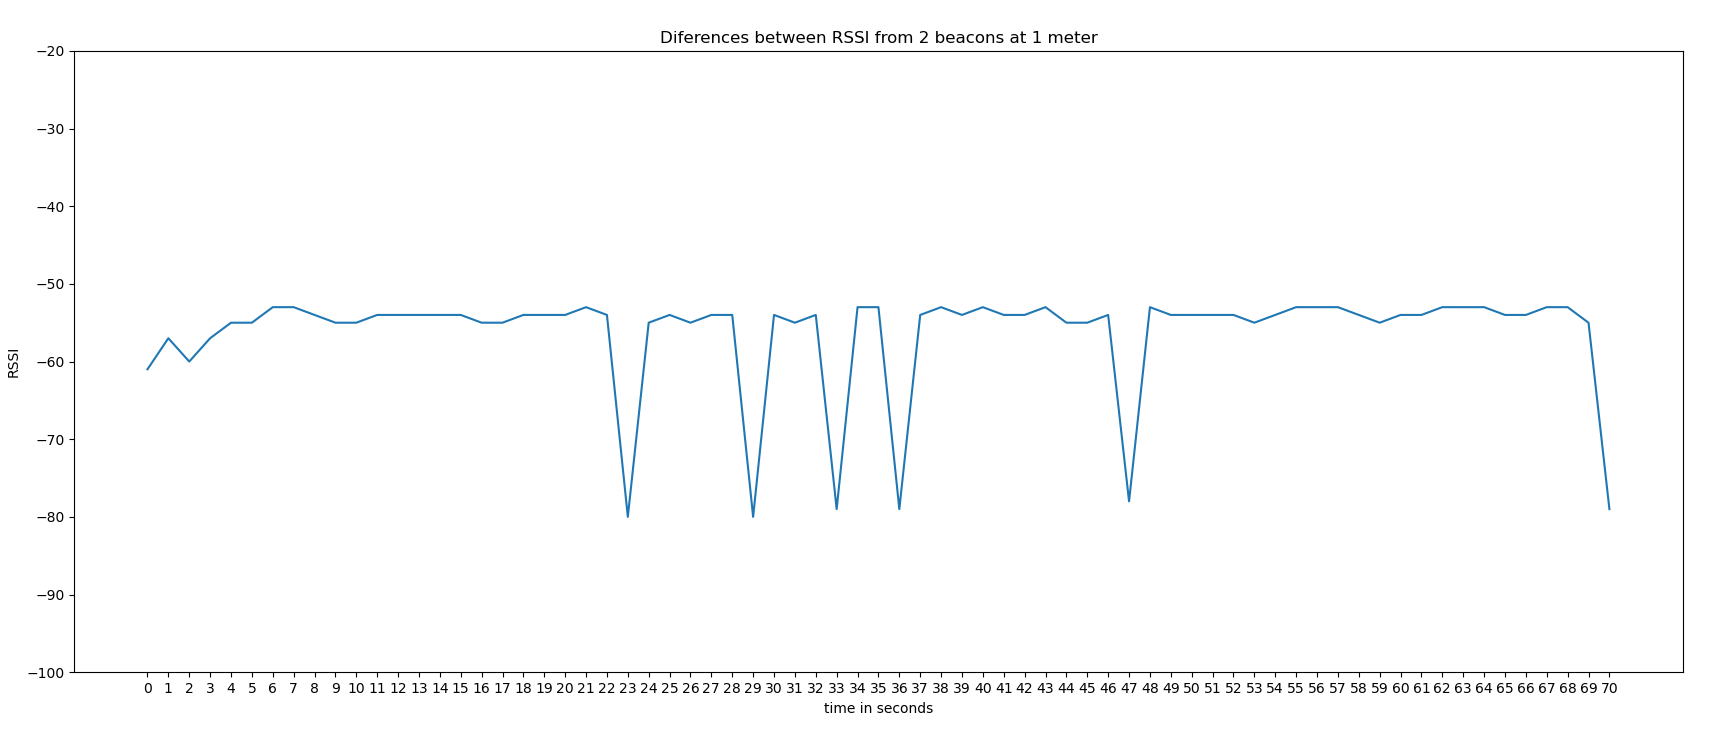
\includegraphics[scale=0.3]{5min_beacon_rssi}
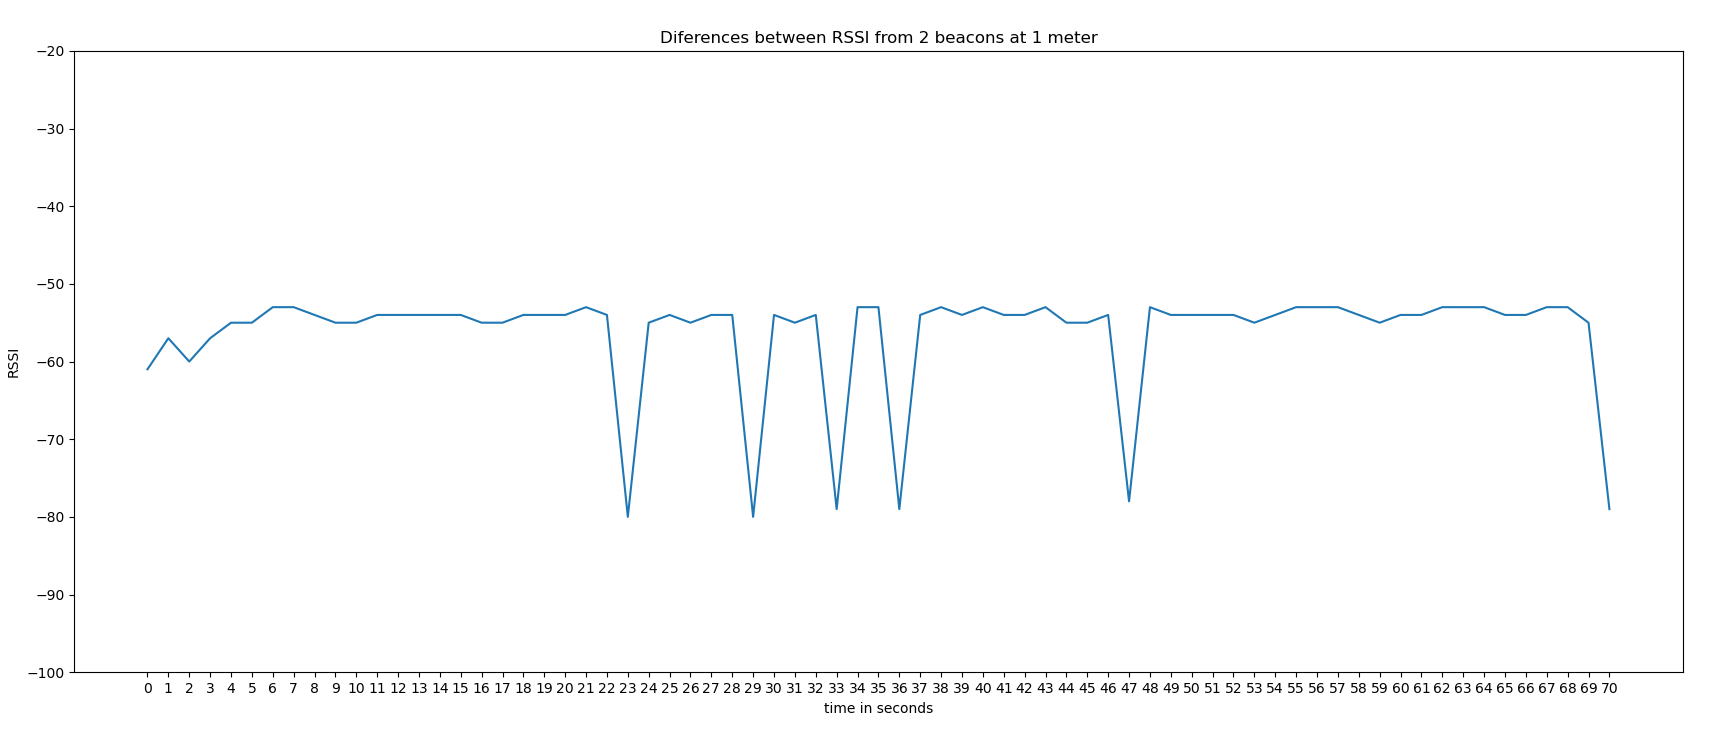
\includegraphics[width=15cm, height=8cm]{5min_beacon_rssi}
\paragraph{hola}
asdfasd

\section{Planos}
\section{Pliego de condiciones y otros documentos legales necesarios}
\section{Presupuestos}
\subsection{test}
\subsubsection{test}


\section{Bibliografía}
\href{https://campus.masterd.es/campusvirtual/index.htm}{Something Linky} 
\begin{itemize}
    \item  yas
\end{itemize}
\begin{enumerate}
    \item  yas
\end{enumerate}
\end{document}